% Physics Behind the Simulation : A CS296 Report by Group 02

\documentclass[english, 11pt]{article}
\usepackage{times}
\usepackage[top=1.0in, bottom=1.0in, left=0.5in, right=0.5in]{geometry}
\usepackage{graphicx}
\usepackage{babel}
%\usepackage{siunitx}

\begin{document}

%Title Goes Here
\title{Physics Behind the Simulation: A CS296 Report by Group 02}

% Author's Name Goes Here
\author{Shubham Jain\\ % Newline
	120050002\\
	shubhamjain@cse.iitb.ac.in\\
	\\	
	Palash Kala\\
	120050010\\
	palashk@cse.iitb.ac.in\\
	\\
	Tapish Raniwal\\
	120050023\\
	tapish@cse.iitb.ac.in\\}

% Today will be replaced with current date
\date{\today}

\maketitle % Without this tag the above information will not appear in the generated document

\section{Introduction}
This report is made as a part of CS296 Assignment 3.
It explains the three new top level blocks defined in the constructor in dominos.cpp. It also explains the phsics behind them.
It describes their motion by considering the conservation equations of the simulation of the blocks.
For learning Box2D we have referred to its official manual\cite{box2dman}.
We have also learned \LaTeX using this tutorial \cite{man1} which we have used for making this tutorial. 

\section{Physics behind the simulation}

\subsection{Box2D top level block 1: The Triangle Wedge}
% Include the physics and atleast one equation (on self line and numbered with units) here. Cite using \cite{cite_key}
The Triangle wedge acts as a wedge and is of triangular shape and is fixed. It is frictionless.
In the simulation it interacts only with the heavy sphere. The heavy sphere collides with it and starts falling down on the wedge.
For finding the state of the system after the collision we have used the law of restitution \cite{book1}\\
\\
Restitution equation: 
 \begin{equation}
 v_a = u \cos(\theta)
 \end{equation}
 \begin{equation}
 v_p = 0
 \end{equation}
 where\\
 $u[{m}{s^{-1}}]$ = initial speed of the sphere (ball) before collision\\
 $\theta[{radian}]$ = angle of collision with the wedge\\
 $v_a[{m}{s^{-1}}]$ = velocity of sphere (ball) along the wedge after the collision\\
 $v_p[{m}{s^{-1}}]$ = velocity of sphere (ball) perpendicular to the wedge after the collision
%\begin{figure}[!ht]
	\begin{center}
		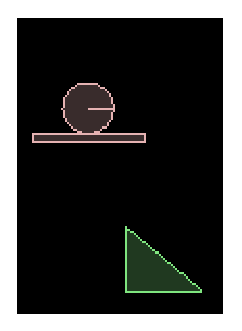
\includegraphics[height=150px]{dominos1}
	\end{center}
%	\caption{New element 1: The heavy sphere ball and Triangle wedge}
%\end{figure}

\subsection{Box2D top level block 2}
% Include the physics and atleast one equation (on self line and numbered with units) here
The old box moves up from sea-saw with a certain velocity and collides with the movable rod attached to the joint.
After collision the box changes its velocity and the rod starts rotating.
For finding these unknown quantities we have used the Newton's laws of motion \cite{book1}
and conservation laws of momentum, angular momentum and energy \cite{book2}\\
\\
Angular Momentum Conservation:
\begin{equation}
\frac{{I_1}{u_p}}{r} = \frac{{I_1}{v_p}}{r} + I_2 {\omega}
\end{equation}
Energy Conservation:
\begin{equation}
\frac{1}{2} {m_1}{u^2} = \frac{1}{2} {m_1}{v^2} + \frac{1}{2} I_2 {\omega}^2
\end{equation}
\begin{equation}
\frac{1}{2} {I_2}{\omega}^2 = {m_2}gh + \frac{1}{2} I_2 {{\omega}_f}^2
\end{equation}
where\\
$I_1[{kg}{m^2}]$  = moment of inertia of box w.r.t. joint\\
$I_2[{kg-m^2}]$ = moment of inertia of rod w.r.t an end\\
$\omega[{s^-1}]$ = angular velocity of rod just after collision\\
$m_1[{kg}]$ = mass of box\\
$m_2[{kg}]$ = mass of rod\\
$u_p[{m}{s^-1}]$ = velocity of box perpendicular to the rod before collision\\
$v_p[{m}{s^-1}]$ = velocity of box perpendicular to the rod after collision\\
$r[{m}]$ = distance of collision from joint\\
$g[{m}{s^-2}]$ = acceleration due to gravity\\
$h[{m}]$ = height from the center of the rod from original position\\
$w_f[{s^-1}]$ = final angular velocity of the rod\\
%\begin{figure}[!ht]
	\begin{center}
		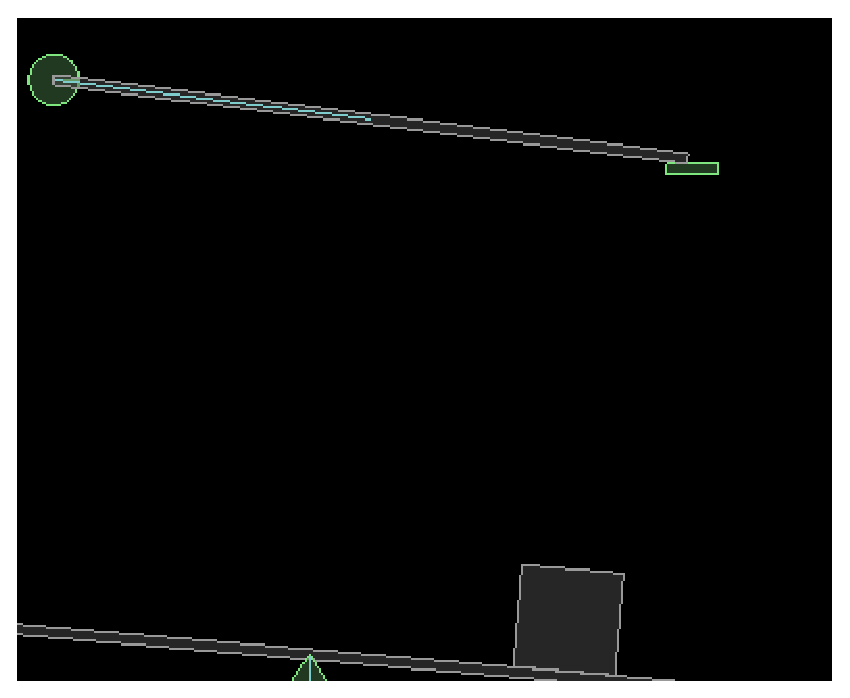
\includegraphics[height=150px]{dominos2}
	\end{center}
%	\caption{New element 2: Box and the revolute joint}
%\end{figure}

\subsection{Box2D top level block 3} 
% Include the physics and atleast one equation (on self line and numbered with units) here
The moving rod hits the box kept at the top of a horizontal shelf. After this the box moves down at a smaller angular velocity.\\
\\
Angular Momentum Conservation:
\begin{equation}
{I_1}{{\omega}_1} = {I_1}{{\omega}_2} + \frac{{I_2}{v_p}}{r}
\end{equation}
Energy Conservation:
\begin{equation}
\frac{1}{2} I_1 {{\omega}_1}^2 = \frac{1}{2} I_1 {{\omega}_2}^2 + \frac{1}{2} m_2 {v_p}^2
\end{equation}
Acceleration:
\begin{equation}
a = g
\end{equation}
where\\
$I_1[{kg}{m^2}]$ = moment of inertia of box w.r.t. joint\\
$I_2[{kg}{m^2}]$ = moment of inertia of rod w.r.t an end\\
$v_p[{m}{s^-1}]$ = velocity of box perpendicular to the rod after collision\\
$r[{m}]$ = distance of collision from joint\\
$m_2[{kg}]$ = mass of rod\\
$a[{m}{s^-2}]$ = acceleration of box after collision\\
$g[{m}{s^-2}]$ = acceleration due to gravity\\
%\begin{figure}[!ht]
	\begin{center}
		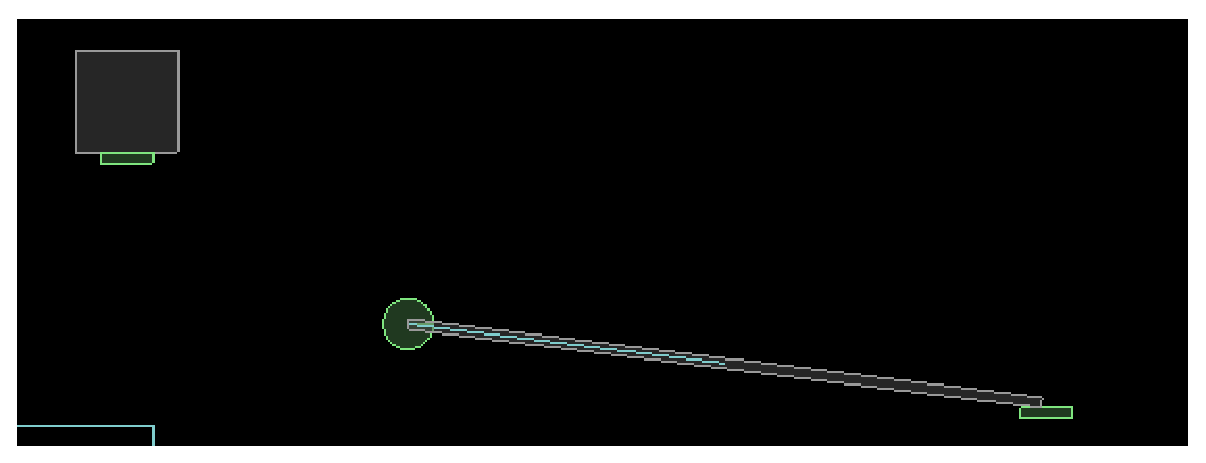
\includegraphics[height=150px]{dominos3}
	\end{center}
%	\caption{New element 3: Revolute joint and the new box}
%\end{figure}

\section{Conclusions} % Summarise the report here
Box2D is an efficient tool for simulation of an ideal physics world.
All the three new block elements have been described above with their equations and in this ideal world they all behave according to these equations.
\bibliographystyle{plain}
\bibliography{cs296_report_02}
\end{document}
